\documentclass{article}
\usepackage[utf8]{inputenc}
\usepackage{graphicx}
\usepackage[hidelinks]{hyperref}
\usepackage{color}
\usepackage{listings}
\usepackage{lastpage}
\usepackage{wrapfig}
\usepackage{eso-pic}
\usepackage{tikz}
\usepackage{float}
\usepackage{pdfpages}
\newcommand{\secref}[1]{\nameref{#1}~\ref{#1}}
\newcommand{\goodcite}[1]{ {(\cite{#1})}}
\usepackage[style=apa, backend=biber]{biblatex}

\setlength\parindent{0pt}

\addbibresource{Ref.bib}

\title{Human Senses and Perception - Mini-Project}
\author{Jannick Drews}
\date{2018}

\begin{document}

\thispagestyle{empty} % REMOVE WHEN DONE
\maketitle
\newpage
\thispagestyle{empty} % REMOVE WHEN DONE
\tableofcontents% REMOVE WHEN DONE
\newpage % REMOVE WHEN DONE
\pagenumbering{arabic} % REMOVE WHEN DONE
% 2000 - 2500 words @ Nov 30 - 23:59
% Discussing the theory relating to HSP,
%     describe how the topics relate to your semester project
% Topics: (See HSP instructions document)
% 1. Illusions
% 2. Somatosensation
% 3. Vection
% 4. Adaptation
% 5. Sound basics
% 6. Auditory streams
% 7. Colour vision
% 8. Depth perception
% 9. Perception in media technology
% 10. Discuss similatiries and diffs between vision and hearing
%     as perceptual systems

\section{Introduction}
\label{sec:Introduction}
This essay will cover aspects of human perception, that relate and are similar to my media technological semester project. This will include the topics; Recognizing visual objects, the gestalt principles and color vision. The semester project revolves around detecting hand postures through color segmentation, in an image and/or video.
\section{Theory}
\label{sec:Theory}

\subsection{Colour vision} % w
%%%%%%%%%%%%%%%%%%%%%%%%%%%%%%%%%%%%%%%%%%%%%%%%%%%%%%%%%%%%%%%%%%%%%
% how is it possible
% Theories on our colour perception
% advantages trichromatic, colour blindness(why it's inaccurate term)
%   , dichromacy advantages
%%%%%%%%%%%%%%%%%%%%%%%%%%%%%%%%%%%%%%%%%%%%%%%%%%%%%%%%%%%%%%%%%%%%%

\subsubsection{Light}
To understand how we perceive color, we must first cover the explanation of light. Light is electromagnetic energy, a stream of photons, with tiny particles which each consists of one quantum of energy, which behaves like a wave\goodcite{hsp}. The property; \textit{wavelength}, defines what color would be perceived by the visual system. An electromagnetic waves wavelength between 370nm to 730nm is typically what humans are able to perceive on the electromagnetic spectrum\goodcite{hsp}, this is displayed on \autoref{fig:EMSpectrum} denoted by the \textit{visible} area of the electromagnetic spectrum.
\begin{figure}[H]
  \centering
  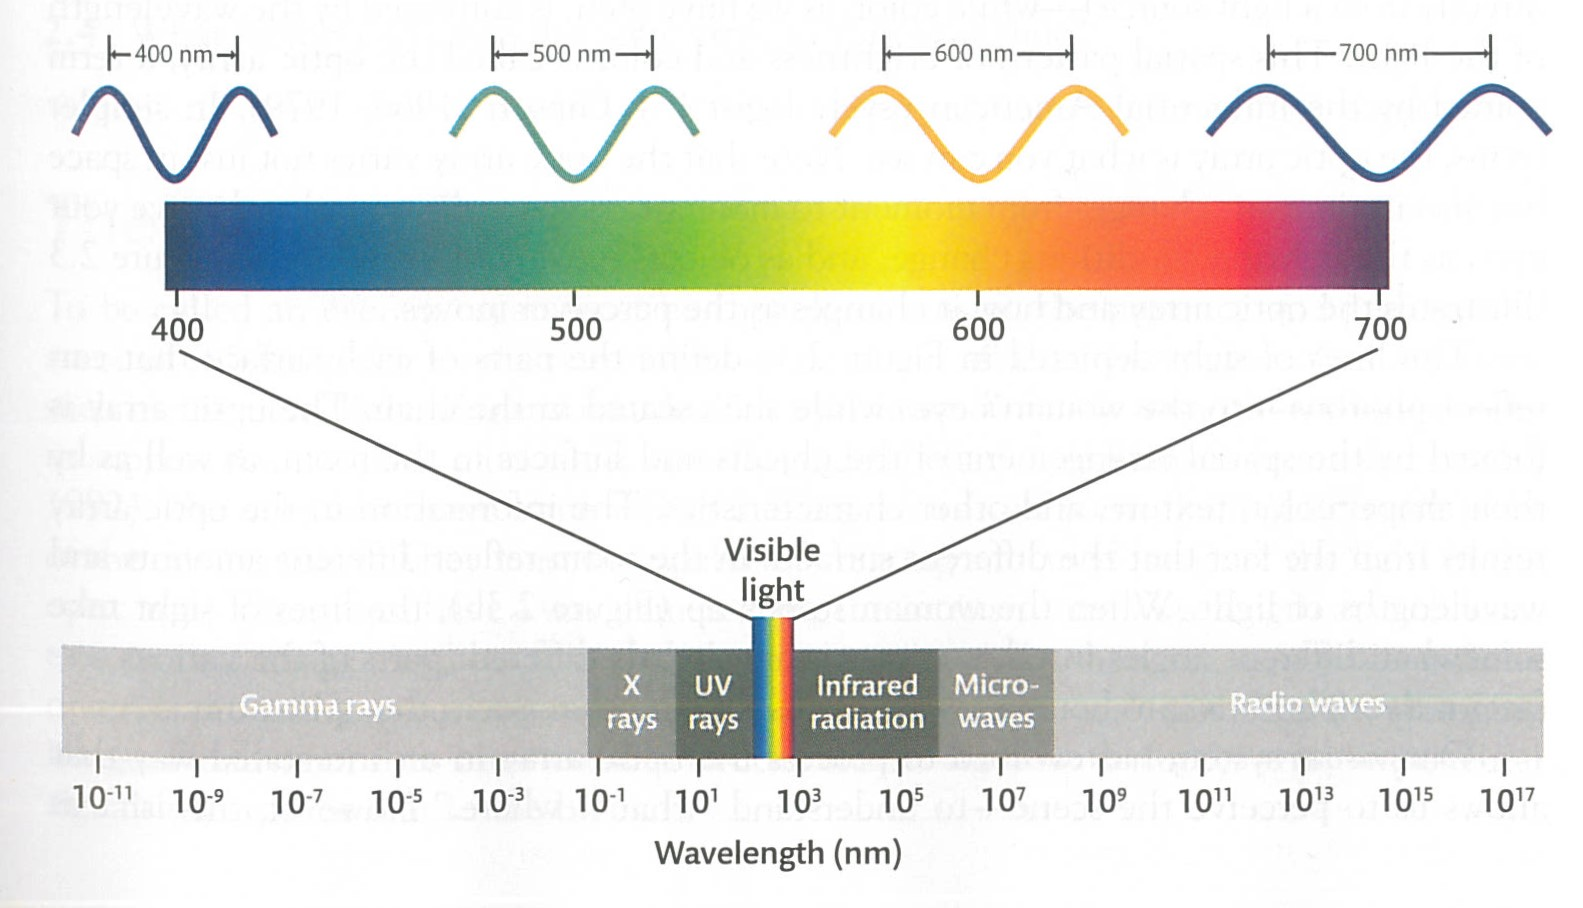
\includegraphics[width=0.8\textwidth]{img/EMSpectrum.jpg}
  \caption{The electromagnetic spectrum\goodcite{hsp}}
  \label{fig:EMSpectrum}
\end{figure}
Even though this explanation is adequate for the physical aspect, there's still different theories on how exactly we will perceive the colors in the spectrum. This will be discussed in \secref{sec:color-trichro-n-dichro}.\\

\subsubsection{Trichromatic \& Opponent-process theory} %TODO
\label{sec:color-trichro-n-dichro}
One evident theory is the Trichromacy theory, which explains that there's three types of cones, each sensitive to their respective wavelength. This is a result of the photosensitive pigment in each of the cones, being sensitive to different wavelengths\goodcite{hsp}.\medskip \\

The opponent-process theory, explains how we typically perceive colours to be off of 4 basic colours; these being: Yellow, Green, Red, Blue\goodcite{hsp}. The reason for this is brain circuits interpreting the receptive signals, and example is the adaptation.

\subsubsection{Light \& The human eye}
Simply, light enters the eye through the Cornea, which then further travels through the Lens past the Iris, the Vitreous chamber and finally arrives at the Fovea, where the light or image is mostly focused\goodcite{hsp}. The Lens and Cornea helps to focus the image and the Iris helps to determine how much light should be let in through the rest of the eye. To focus the image, the Lens help to refract the light, to make sure the light is properly focused, when it reaches the retina\goodcite{hsp}.\medskip \\

\begin{figure}[H]
    \centering
    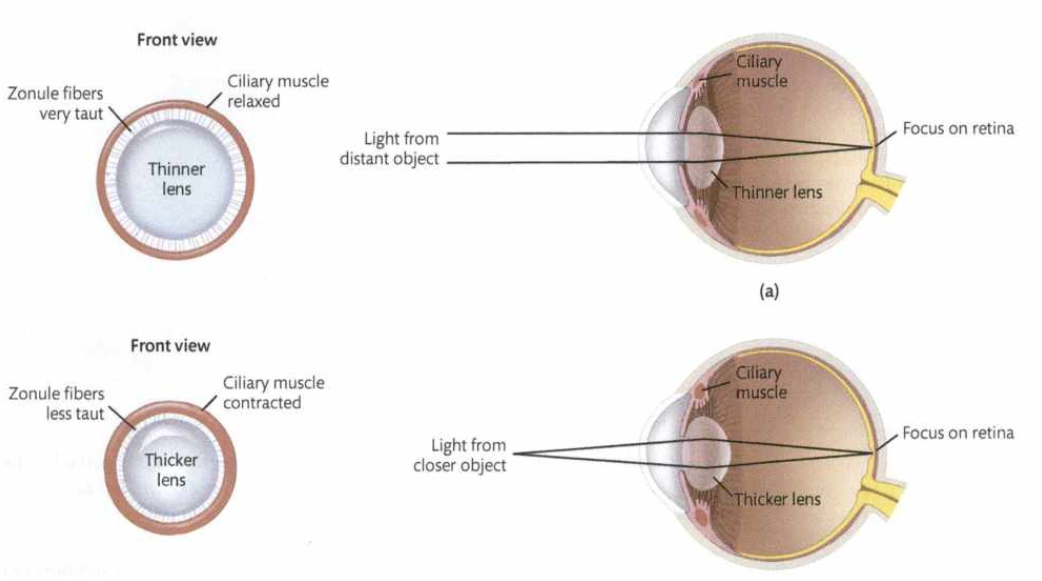
\includegraphics[width=\textwidth]{img/eyelens.png}
    \caption{Focusing light in the eye\goodcite{hsp}}
    \label{fig:focus_light}
\end{figure}

Adjusting the shape of a lens, the focal point can be altered and thereby determining the position of where the lightrays should focus. The Lens in the eye will be stretched by muscles in the eye, to focus on objects that are at different distances, see \autoref{figu:focus_light}. This specific adjustment in the lens and eye is called \texttt{accomodation}\goodcite{hsp}.

\subsubsection{Photoreceptors}
The photoreceptors in the eyes retina consists of rods and cones, which are two types of neurons which transduce light into neural signals. The cones carry the information of the difference in wavelength, whereas the rods do not carry much information in regards to wavelength but are much more sensitive to the intensity of light\goodcite{hsp}.\\After the light has been converted into neural signals, they get propagated to multiple other cells and finally to the retinal ganglion cells, which axons bundle together and send action potentials(AP) to the brain\goodcite{hsp}.\\

\subsubsection{Cameras \& Digital sensors}
Similar to an eye, the lens of a camera aim to duplicate the functionalities for getting a sharp and clear image(REF). More specifically, an important factor in optical systems is the lens, which serves to focus incoming light, typically onto a set of sensors\goodcite{IP}.\medskip\\ % NEED MORE TODO

\begin{figure}[H] % REPLACE ME TODO
    \centering
    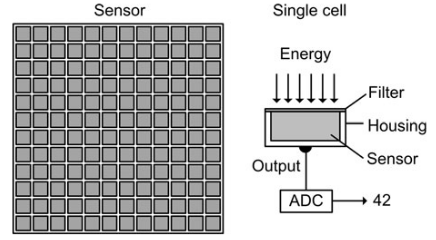
\includegraphics[width=0.8\textwidth]{img/sensor.png}
    \caption{Image sensor\goodcite{IP}}
    \label{fig:Image_sensor}
\end{figure}

The digital sensors created for storing electromagnetic waves as energy behaves like how the rods and cones in the retina stores/charges(MAKE SURE) the electromagnetic waves, and more specifically the amount of charge depending on the specific wavelength of the wave.\\The digital sensor is although suited with a grid-system of red, green and blue wavelength sensitive sensors, which will then convert the retrieved wave energy into a 2D-image. This resembles how the retina also constructs an image from the rods and cones, which are sent further to the brain by the ???Ganglion cells??? %TODO

%%%%%%%%%%%%%%%%%%%%%%%%%%
%%%%% Next Topic %%%%%%%%%
%%%%%%%%%%%%%%%%%%%%%%%%%%

%\subsection{Somatosation} % w/2
%\subsubsection{Proprioception \& Kinesthetic}

%\subsection{Perception in media technology} % w

\subsection{Recognizing visual objects}% w * 2
Recognizing objects might be a simple task for a human, but it shows to be a lot more than just visually perceiving an object. Multiple elements play a role in proper object recognition, such as Figure-Ground organization, Perceptual grouping, Perceptual interpolation, recognition by components mode, edge detection and the Gestalt principles.\\medskip \\
%\begin{figure}
%    \centering
%    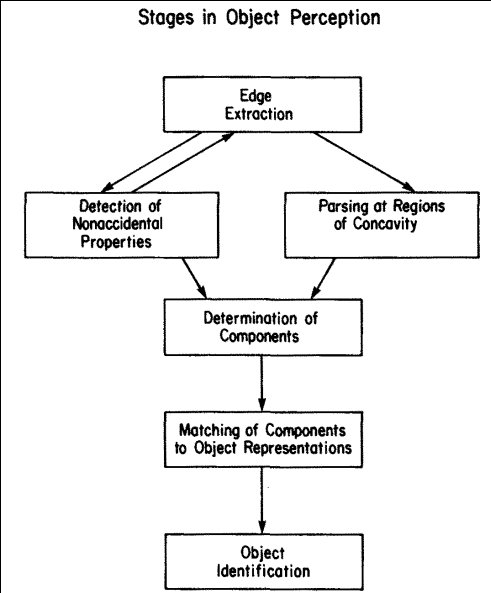
\includegraphics[width=0.5\textwidth]{img/ObjectSteps.png}
%    \caption{Stuff}
%    \label{fig:ObjectHiarchy}
%\end{figure}
The steps for recognizing visual objects is split into two layers, firstly the perceptual organization which generally includes the pattern of neural activity to represent edges and regions, dividing these regions and grouping them with similar properties whilst at the end filling in missing elements. The second layer being the object recognition, which matches the candidate objects to the representations stored in memory\goodcite{hsp}\goodcite{bieder}.

\subsubsection{Perceptual Organization}
\label{sec:perceptialorganization}
Perceptual organization serves to make object recognition in complex scenes possible, it does this by "detecting" edges and regions in a retinal image and performing a certain amount of steps to further candidate objects in the scene, for later recognition\goodcite{hsp}.\\
Three complications are quite important, when talking about the analysis of object recognition, these three can be pronounced like the following; image clutter, object variety and variable views.\\
Image clutter refers to the fact that multiple objects in a scene may occlude each other, where the visual system must make up for the occluded parts of objects. The object variety refers to how many different objects there is it generally recognize, this is in terms of shape and form. Even if the object is difficult to specifically identify, a general idea of what the object is can still be found. Variable views, is how an object appearing differently on the retinal images, depending on the orientation and the viewpoint of the object whilst also being of different illumination\goodcite{hsp}.\\

% THIS CAN BE RELATED TO THE SEMESTER PROJECT IN TERMS OF HAND EDGES AND REGION(BLOB ANALYSIS & EDGE DETECTION(CONVEX HULL))
The edges and regions are "detected" by patterns of neural activity, responding to location, orientation and curvature of objects in a simple scene. This can be more abstract when reviewing an image of more complex intensity of brightness, and example could be any scene with occlusion, shadows or shading on an object which also refers to the previously used term; image clutter. The question then becomes, how can the brain then resolve the complex or cluttered scenes?\\
% NOW RELATE TO PROJECT %TODO
% blabla image processing

% MORE ABOUT HSP
The question can be answered by covering multiple topics which makes up good candidates for the second layer of recognizing visual objects. Firstly dividing the regions into figure and ground, to explain this simply, its the identification of a figure from a background, in terms of the Gestalt psychology or more specifically, a type of perceptual grouping in the Gestalt Principles. The figure and ground Organization is only one of multiple perceptual grouping techniques used to identify figures in a scene.\goodcite{hsp}\\

\begin{figure}[H]
    \centering
    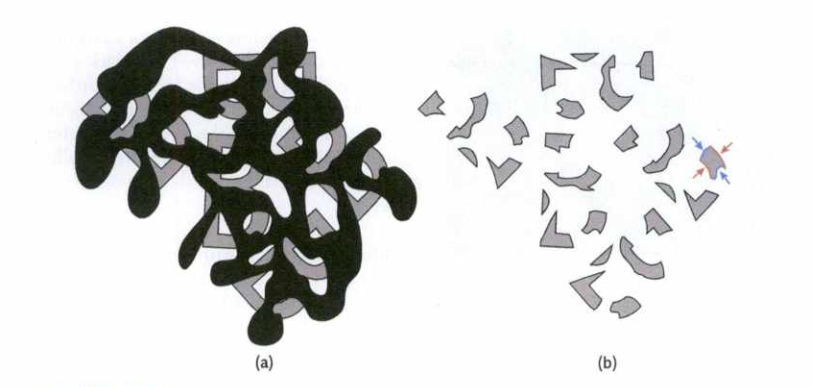
\includegraphics[width=\textwidth]{img/b.png}
    \caption{Illustration of Border Ownership and Figure-ground Organization\goodcite{hsp}}
    \label{fig:border_ownership}
\end{figure}

\autoref{fig:border_ownership} illustrates the grouping technique of border ownsership and figure-ground organization, on the left figure (a) it's easier to determine the borders and therefore easier to determine the occluded letters B. Whereas on the right figure (b), it's harder since the visual system gives all the fragment borders ownership (Which makes them seem like individual figures).\medskip \\

%\subsubsection{Recognition by- componets or specific viewpoints}
%A problem that... %blablalba WRITE, although what can it relate to

\subsubsection{BLOB Analysis}
A likely media-technological relative to the figure-ground organization could be BLOB(Binary Large OBject) analysis, which is a technique in Image Processing. BLOB analysis is the extraction, feature and classification of a BLOB, in an image\goodcite{IP}. The BLOB will then be classified as an arbitrary object in the image\goodcite{IP}.\\It does this by going pixel by pixel of an image, and then marking the pixels as objects, the determination of which pixels belong to what object is determined by the kernel used\goodcite{IP}.\medskip \\

Referring to the \autoref{fig:border_ownership} again, the BLOB analysis would to a certain extent, also arrive at the same result as the average human would perceive. Since the right figure (b), where the fragments have no interconnection, the BLOB analysis would regard all the fragments as individual BLOBs, whereas the right figure (a) would be determined as one whole (keeping in mind that the ink would have to be the same color as the occluded letters).\\Another candidate for a media-technological relative to the figure-ground organization, more specifically detecting edges from intensity of color and/or brightness, could be Thresholding. Thresholding is the process of mapping a certain range of pixels with a specific pixel-value to either 0 or 255, or 0 and 1\goodcite{IP}. Thresholding takes a specific thresholding value, which it then compares to all the pixels of an image. If the pixel-value is lower than the threshold value then it assigns the pixel-value to 0 whilst the reverse operation is applied to pixel-values above the threshold value\goodcite{IP}. This will help segment figures that are of different color and/or brightness from the rest of the image clutter.


\subsubsection{Gestalt principles}
Proximity, common fate, similarity
%Object recognition
%Edge completion?

\subsubsection{Object recognition}
After the creation of candidate objects by the perceptual organization steps, the visual system now has to recognize the objects. This is done by matching the objects, to stored memory in the brain.\\

\begin{center}
\textit{"Core object recognition is the ability to rapidly discriminate a given visual object from all other possible visual objects without any object-specific or location-specific pre-cuing"}\goodcite{solveVisual}\\
\end{center}

It makes sense to claim that the visual system must somehow be able to compare objects to memory, despite changes in viewpoints of said object. A visual system that can achieve this, exhibits \textit{invariance}\goodcite{hsp}.\\There are different approaches to how invariance is achieved by the visual system, one of them being the recognition by components model. This model is built on how object recognition depends on; \textit{"identifying the primitive geometrical components that make up the object"}\goodcite{hsp}.\\This is illustrated on \autoref{fig:components}, by looking at figure (c) and figure (d), it is clear how the location of the handle denotes whether the object is a cup or that of a bucket.

\begin{figure}[H]
    \centering
    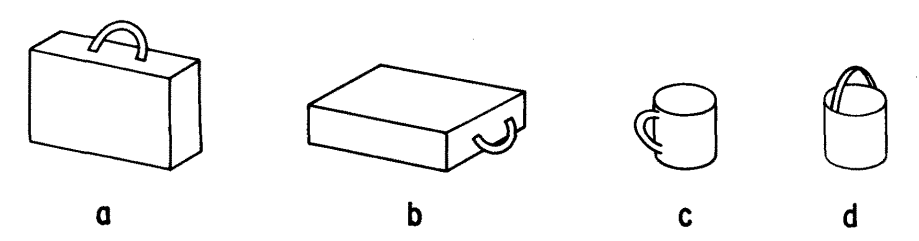
\includegraphics[width=\textwidth]{img/comps.png}
    \caption{Different arrangement of components produce different objects.\goodcite{bieder}}
    \label{fig:components}
\end{figure}


Another approach to invariance, is that it is based on a view-specific manner, in which multiple representations of a single object would be stored.\medskip \\ % TODO

\subsubsection{Feature - \& Template matching}
Computer-vision specific technologies that exhibit partwise the same traits as the view-specific manner of approaching invariance, is the feature matching. Template matching does however give a rough estimate of how much a candidate object matches the stored representation, altough viewpoint and similarity is a big factor in this type of matching.\\Feature matching takes certain features of an object and matches it against objects in a scene and retrieves the most likely match based on distance calculations\goodcite{OpenCV}.

% Medialogy related problems. Give at least three examples of technological advancements, where knowledge of human perception has been (or would be crucial) for the technological advances. How was the innovation

% Comments about object recognition theories
% Invariance, constancy, two theories(suggestions) critics on second theory
% First theory very abstract
% - We store generalized small objects and depending on the combination of the simple objects, we form a greater object to recognize, this is also affected by the viewpoint
% -
% Second theory
% - We store all information about an object, how we match it depends on the similarity of the images, e.g. 3 angles of a car are very similar = same object.

\section{Discussion \& Conclusion}
% Color & Eye vs Camera & Digital Sensors
% BLOB & Thresholding vs Perceptual Organization
% Feature matching vs Object Recognition
% TODO
\newpage
\section{Bibliography}
\label{sec:Bibliography}
\printbibliography

\end{document}
